\documentclass[18pt, a3paper, portrait]{tikzposter}
\usepackage[utf8]{inputenc}

\makeatletter
\def\title#1{\gdef\@title{\scalebox{\TP@titletextscale}{%
\begin{minipage}[t]{\linewidth}
\centering
#1
\par
\vspace{0.5em}
\end{minipage}%
}}}
\makeatother

\title{Data Exploration, Discussion and Conclusion}
\author{Yohann Jacob Sandvik}
\date{\today}
\institute{Institute of Electronic Systems - NTNU}
 
\usepackage{blindtext}
\usepackage{comment}
\usepackage{tikz} % To make cool diagrams
\usepackage{booktabs} % For fancy tables

\newcommand{\ra}[1]{\renewcommand{\arraystretch}{#1}} % Something about allowing more space between rows in fancy tables.
 
\usetheme{Envelope}
 
\begin{document}
 
\maketitle 

%% Dataset description
\begin{columns}
    \column{0.5}
    \block{All Values Associated with A Turbine}
    {
        \begin{tikzfigure}
            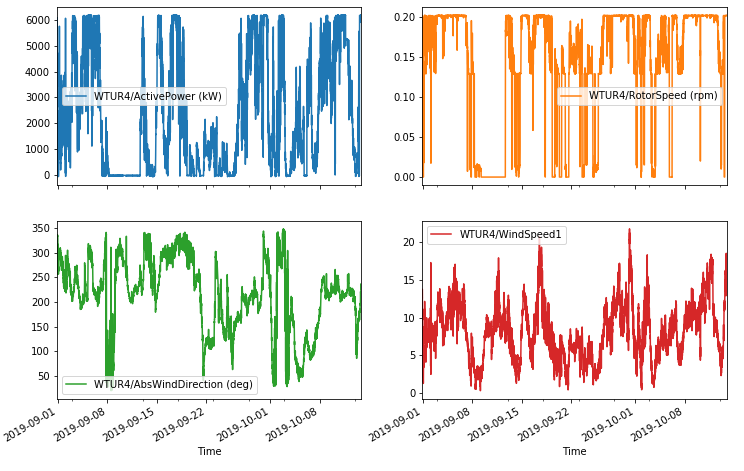
\includegraphics[width=0.45\textwidth]{images/one_turbine_all_vals.png}
        \end{tikzfigure}
    }
 
    \column{0.5}
    \block{Dataset Description}
    {
        \begin{itemize}
            \item This dataset is taken from a wind farm in Norway with 13 wind turbines.
            \item Each turbine can be viewed as a multivariate time series, with four dimensions: active power produced by a turbine in kilowatts, wind speed measured in front of the blades in meters per second, the rotational speed of the rotor in rpm and the absolute direction of the wind speed in degrees.
            \item The values are sampled every five minutes from the 31. of August 2019 00:00 until the 13. of September 2019 21:55, which totals 12239 samples per univariate time series and 48956 samples per wind turbine.
            \item The dataset chosen does not have any missing values, so there was no requirement for estimating missing values.
        \end{itemize}
        \vspace{4cm}
    }
\end{columns}

%% Describe tool and show figures of explained variance, and reconstruction error
\begin{columns}
    \column{0.5}
    \block{}
    {
        Text and more text. I want to add a new line. \newline
        Did it work?
        \vspace{4cm}
    }
 
    \column{0.5}
    \block{}
    {
        Here,  
        \vspace{4cm}
    }
\end{columns}

%% Artificial perturbation pics
\begin{columns}
    \column{0.25}
    \block{}
    {
        Here,  
        \vspace{4cm}
    }

    \column{0.25}
    \block{}
    {
        Here,  
        \vspace{4cm}
    }

    \column{0.25}
    \block{}
    {
        Here,  
        \vspace{4cm}
    }

    \column{0.25}
    \block{}
    {
        Here,  
        \vspace{4cm}
    }
\end{columns}

%% Discussion 
\block{Final Discussion}
{
    THIS IS THE DISCUSSION, OR IS IT?
}

%% Conclusion and future work
\block{Conclusion}
{
    THIS IS THE CONCLUSION.
}
\end{document}


